\subsection*{Presentación}
En esta sección, presentamos las pruebas experimentales sobre las implementaciones de los filtros, los resultados obtenidos en cada una de ellas y comentarios sobre los mismos. El objetivo de esta sección es evaluar y comparar el rendimiento de las diferentes implementaciones y así obtener conclusiones acerca de las características del modelo de programación SIMD.

\subsection*{Metodología}

En nuestros experimentos, buscamos realizar una comparación de performance de las implementaciones de cada filtro para sus versiones en C y en ASM.
Las versiones de C fueron compiladas utilizando el nivel de optimización \textbf{O3}, ya que realizando mediciones preeliminares observamos que la cantidad de clocks utilizados, para cada una de estas, era mucho menor con ese nivel de optimizacion y dado el objetivo de buscar superar en rendimiento a las versiones de C con las de ASM optamos por comparar con las de mejor velocidad posible.
Por otro lado, intentamos que no difieran demasiado los algoritmos entre las implementaciones de C y ASM, en cuanto a las secuencia de acceso a datos, y los tipos de datos utilizados para guardar los valores, para de esta forma tener una comparacion que refleje lo mas fielmente posible la ventaja de utilizar instrucciones SIMD.

Para realizar las mediciones hemos modificado el programa tp2.c para realizar una medición de tiempo por cada aplicación de filtro, ademas desarrollamos scripts en python para poder automatizar las ejecuciones y la recoleccion de resultados, y asi poder analizar los resultados de una forma consistente y reproducible, tanto en diferentes maquinas como luego de modificar los filtros. 

Para hacer las comparaciones, decidimos utilizar el minimo de ejecutar 100 veces el mismo filtro, luego de haber observado que el histograma generado por las ejecucion de 500 veces el mismo filtro generaba una mayor cantidad de resultados cerca del minimo, y luego de analizar que tenia sentido comparar la minima cantidad de clocks utilizados por un filtro y de esta manera descartar la mayor cantidad posible de interferencias producidas por el sitstema opertaivo.

\begin{figure}[!h]
	\centering
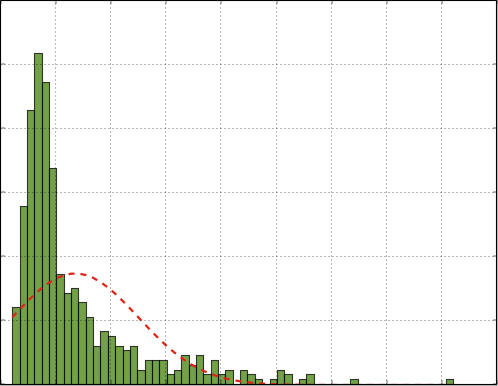
\includegraphics[width=200px]{imgs/distribucion.png}
\end{figure}


De esta forma, hemos realizado las mediciones de tiempos sobre nuestras implementaciones utilizando imágenes de distintos tamaños. Realizamos 2 analisis diferentes, uno utilizando imagenes con un mismo ancho o un mismo alto pero incrementando la otra componente, y comparando estos valores para una misma implementacion, con el fin de observar si se generaban resultados diferentes para una misma cantidad de pixeles pero con diferente organizacion. 

Para el segundo analisis y con el cual realizamos la comparación entre diferentes implementaciones utilizamos imagenes de tamaño creciente para poder observar si para diferentes cantidades de pixels los filtros mantenian la misma relacion de velocidad.
Las dimensiones utilizadas para el primer analisis fueron imagenes de 16x16*2$^{i}$ y 16*2$^{i}$x16 y para el segundo de 16*2$^{i}$x16*2$^{i}$ (con 0 $\leq$ i $\leq$ 9)

\newpage
\subsection{Cropflip}
\subsubsection{Hipótesis}
Para este filtro en particular no teniamos una idea predefinida de con que resultados nos ibamos a encontrar al realizar la experimentacion.
Al ser este un filtro muy sencillo sin necesidad de realizar operaciones matematicas en las cuales poder operar con muchos pixeles en simultaneo, la hipotesis era que la diferencia iba a estar dada por la forma de acceder a memoria pero sin esperar significativas diferencias entre una version y otra.

Elegimos tambien agregar 2 versiones extra de asm: una para medir el acceso mas simple pixel a pixel, y otra utilizando operaciones de repeticions para copiar strings, que para este caso tenia sentido aprovechar.

\subsubsection{Resultados obtenidos}

De estos resultados pudimos sacar algunas concluciones, por un lado la version de C funciono marginamlente mejor que la version asm byte a byte, por lo cual suponemos que, por lo menos en funciones en la cuales la cantidad de instrucciones dentro del ciclo es minima, no hay mucho lugar a optimizaciones posibles y el resultado es un poco mejor debido a algun mejor manejo de las variables utilizadas para iterar.

Por otro lado la version que mejor funciono fue la que utiliza la instruccion rep del microprocesador, obteniendo una ganancia del 34\% respecto a la version optimizada de C.
Incluso funciono mejor que la version simd que procesa de a 16 bytes juntos, pero que requiere mas cantidad de instrucciones para realizarlo.

De todas formas la version que utiliza simd funciono 12\% mas rapida que la version  de C con o3.


\begin{table}[!htbp]
	\centering
	\footnotesize
	\begin{tabular}{| c | c | c | c | c |}
		\hline
Pixels &asm (rep movsb)& asm (simd) & c (o3) & asm (byte a byte)\\ \hline
16x16 & 519 & 492 & 608& 821 \\ \hline
32x32  &1319  & 1594 & 2385& 2859\\ \hline
64x64  & 4430 & 5811 & 9398& 10880 \\ \hline
128x128 & 17508 & 22199 & 40104& 42483 \\ \hline
256x256  & 74415  & 100670 & 158598& 173322\\ \hline
512x512   & 272945 & 406759 & 630169& 685997 \\ \hline
1024x1024 & 2374453 & 2142237 & 4106284& 3088009 \\ \hline
2048x2048  & 10541158  & 14051375 & 15710302& 15923283\\ \hline
4096x4096 & 42235970 & 56320833 & 64179899& 65792957 \\ \hline
8192x8192 & 168890652 & 228391061 & 259152207& 266746729 \\ \hline
Tiempo en X& 1x & 1.35x & 1.53x & 1.57x  \\ \hline
Ganancia vs C & 34.83\% & 11.87\%	& 100.00\% & -2.93\% \\ \hline

 
	\end{tabular}
\end{table}


Es interesante ver que en la version con rep, como evoluciona la cantidad de clocks utilizados para procesar una imagen con la misma cantidad de pixels, pero difere si crece en ancho de si crece en alto.
Debido a que la funcion rep solo se aplica para copiar filas, se ve en la imagen como esta optimizacion mejora su relacion a medida que crece el ancho.

\begin{figure}[!h]
	\centering
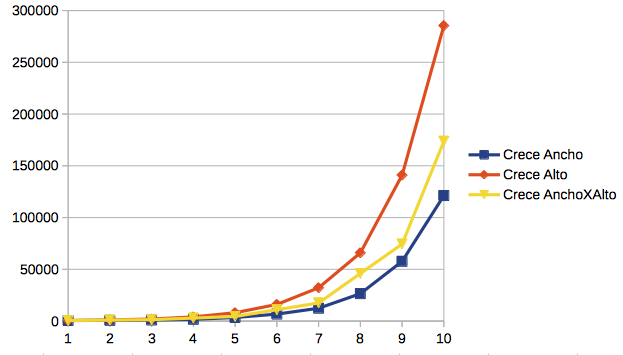
\includegraphics[width=250px]{imgs/crecimientocrop.png}
\end{figure}





\newpage
\subsection{Sepia}
\subsubsection{Hipótesis}

Para este filtro esperamos observar, como primer analisis, que las implementaciones tengan un crecimiento estable a medida que van creciendo una misma cantidad de píxeles pero con diferente organización.

Como segundo analisis, creemos que las implementaciones realizadas en ASM sean mas eficientes que la realizada en C, sin importar el tamaño de la entrada, ya que la implementación en C procesa los pixeles de manera independiente y ambas implementaciones en ASM utilizan operaciones del formato \textbf{SSE} y procesan más píxeles al mismo tiempo.

Entre las dos implementaciones de ASM, esperamos que la implementación ASM 2 (\textbf{sepia_asm2.asm}) sea levemente más eficiente frente a la implementación ASM 1 (\textbf{sepia_asm.asm}) ya que posee una operación menos para realizar los calculos sobre los pixeles y no posee una operación de división (\textbf{divps}), que si posee ASM 1.

\subsubsection{Resultados Obtenidos - Primer Analisis}

Los siguientes graficos presentan los resultados obtenidos de nuestro primer analisis en donde realizamos la comparación de cada una de las implementaciones consigo misma con el fin de observar si se generan resultados diferentes para una misma cantidad de píxeles pero con diferente organización.

\begin{figure}[h!]
	\centering
		\begin{tabular}{cc}
		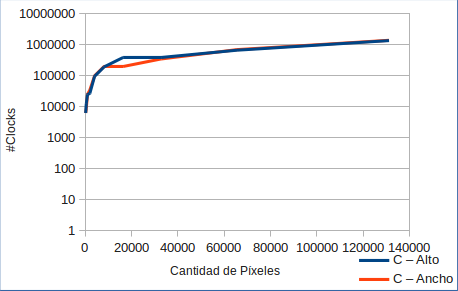
\includegraphics[width=250px]{imgs/sepia-c-analisis1.png} &
		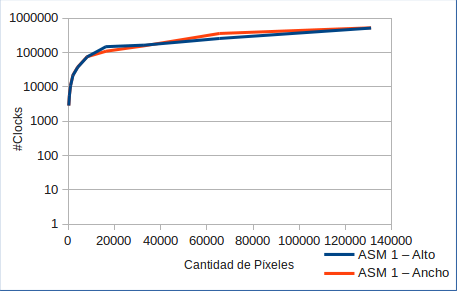
\includegraphics[width=250px]{imgs/sepia-asm1-analisis1.png} \\
		\end{tabular}
		\begin{tabular}{c}
		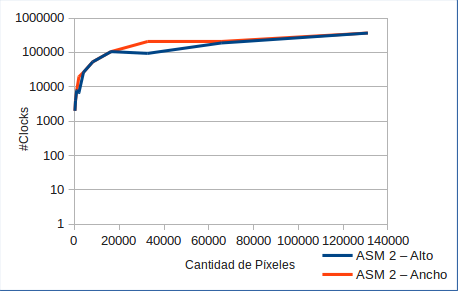
\includegraphics[width=250px]{imgs/sepia-asm2-analisis1.png} \\
		\end{tabular}
\end{figure}

Podemos observar que las curvas de crecimiento de nuestras tres implementaciones del filtro tienden a tener un mismo comportamiento a media que la cantidad de pixeles va en aumento, lo que afirma nuestra hipótesis sobre este primer analisis. Por otro lado, también puede observarse que para tamaños de entrada de entre 20000 y 40000 píxeles las tres implementaciones generar una diferencia, en alguno mas sutil como en ASM 1 y en otro mas marcada como en la de ASM 2. Este comportamiento inesperado sería interesante estudiarlo posteriormente.

\subsubsection{Resultados Obtenidos - Segundo Analisis}

Los siguientes graficos presentan los resultados obtenidos de nuestro segundo analisis en donde realizamos la comparación de performance de cada una de las implementaciones con las demás.

\begin{figure}[h!]
	\centering
	\begin{tabular}{ll}
		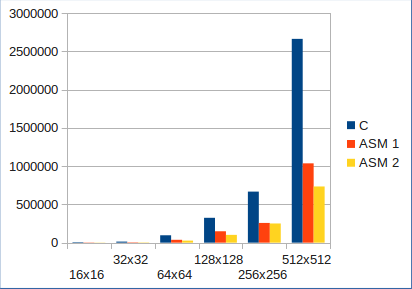
\includegraphics[width=250px]{imgs/sepia-analisis2-1.png} & 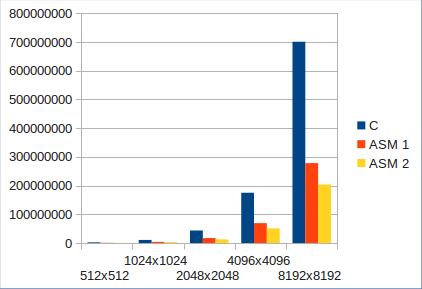
\includegraphics[width=250px]{imgs/sepia-analisis2-2.png} \\
		\vspace{1em}
	\end{tabular}
\end{figure}

Como podemos observar, la implementación en C (con O3) resultó ser mucho menos eficiente que sus contrapartes de ASM (que obtubieron ganancias del 70\% y 80\% con respecto a la implementación en C), a medida que la imagen va creciendo, esto afirma nuestra primera parte de la hipotesis. Por otro lado, entre los algoritmos ASM 1 y ASM 2 pudimos observar que se obtuvo una mas pequeña mejora en performance del ASM 2 sobre ASM 1. Esto afirma nuestra segunda parte de la hipotesis, las operaciones de división y sumas que posée la implementación ASM 1 son mucho mas costosas que las multiplicaciones que posée la implementación ASM 2 y esto se refleja en la diferencia de 0.36x superior en el tiempo de ejecución de ASM 1 con su contraparte ASM 2.

\begin{table}[!htbp]
	\centering
	\footnotesize
	\begin{tabular}{| c | c | c | c |}
		\hline
Pixels &ASM 2 & ASM 1 & C (O3) \\ \hline
16x16 & 1996 & 2862 & 6278 \\ \hline
32x32  &4232  & 4869 & 13580 \\ \hline
64x64  & 26383 & 37273 & 96682 \\ \hline
128x128 & 101613 & 148681 & 324678 \\ \hline
256x256  & 250612  & 257940 & 667089 \\ \hline
512x512   & 733971 & 1036902 & 2664477 \\ \hline
1024x1024 & 3161181 & 4314780 & 10863381 \\ \hline
2048x2048  & 12802011 & 17375403 & 43898460 \\ \hline
4096x4096 & 51152475 & 69574692 & 175335426 \\ \hline
8192x8192 & 204137541 & 278365320 & 700733874 \\ \hline
Tiempo en X& 1x & 1.36x & 3.43x \\ \hline
Ganancia vs C & 70.86\% & 60.29\%	& 100.00\% \\ \hline

	\end{tabular}
\end{table}

\newpage
\subsection{Low-Dyn Range}
\subsubsection{Hipótesis}

Para este filtro en particular, dada su complejidad, en cuanto al orden necesario para acceder en memoria a los valores, y los calculos para arrivar al resultado, hipotetizamos que la diferencia obtenida entre la mejor version de ASM y la mejor version de C serian mayores que las mismas comparaciones entre otros filtros, debido a que las optimizaciones que el compilador pudiese efectuar sobre el codigo y los accesos a memoria, no serian tan buenas como hacer un analisis especifico del funcionamiento del filtro y deduciendo que valores se puede reutilizar y que calculos se pueden realizar en paralelo utilizando instrucciones SSE.

Por otro lado realizamos 2 versiones diferentes tanto en C como en ASM con la idea de poder comparar por un lado la ganancia posible a travez de instrucciones SSE y por otro la gananica de reordenar la forma de acceso a los datos.


\subsubsection{Resultados obtenidos}


Los resultados que obtuvimos estuvieron razonablemente dentro de lo esperado. La ganancia entre la mejor version de ASM y la mejor de C con optimizacion en O3, permitiria aplicar el filtro en un poco mas de 4 imagens al mismo tiempo que la de C se lo aplica a 1 sola, o tambien, pudiendo aplicar el filtro a una imagen del doble de ancho y doble de alto (lo cual es muy util en el contexto de pantallas cada vez con mas resolucion). 

Tambien de alguna manera esperado fue que la ganancia utilizando SIMD fuese de ~4x dado que es justamente la cantidad de pixels que se pueden manejar simultaneamnte .

\begin{table}[!htbp]
	\centering
	\footnotesize
	\begin{tabular}{| c | c | c | c | c | c |}
		\hline
Pixels & ASM & C (o3) & C preproc (o3) & ASM simd & ASM simd preproc \\ \hline
16x16  & 33357 & 18596 & 13153 & 5194 & 3449 \\ \hline
32x32  & 181961 & 101292 & 62862 & 27944 & 15221 \\ \hline
64x64  & 837330 & 465902 & 289280 & 134856 & 65339 \\ \hline
128x128  & 3574572 & 1995407 & 1231802 & 548901 & 272744 \\ \hline
256x256  & 14911141 & 8238530 & 5276382 & 2274634 & 1159197 \\ \hline
512x512  & 61337662 & 34614421 & 22898444 & 9514187 & 4865965 \\ \hline
1024x1024  & 246805935 & 135432773 & 85989437 & 38506702 & 20900364 \\ \hline
2048x2048  & 996559614 & 547159461 & 348591233 & 156452341 & 90032611 \\ \hline
4096x4096  & 4139577580 & 2273534155 & 1566227645 & 639810532 & 363950690 \\ \hline
8192x8192  & 16999317092 & 9493848236 & 6354314134 & 2644797660 & 1533749148 \\ \hline
Relacion & 11.0835054834 & 6.1899615386 & 4.1429944018 & 1.7244004102 & 1 \\ \hline

	\end{tabular}
\end{table}


\begin{figure}[!h]
	\centering
	\begin{minipage}{.5\textwidth}
		\centering
		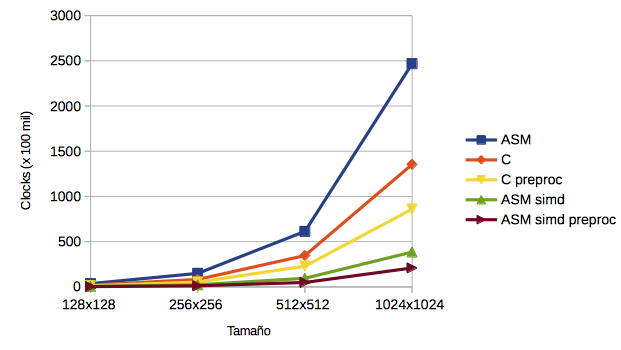
\includegraphics[width=\linewidth]{imgs/ldrTotales1.png}
	\end{minipage}\hfill
	\begin{minipage}{.5\textwidth}
		\centering
		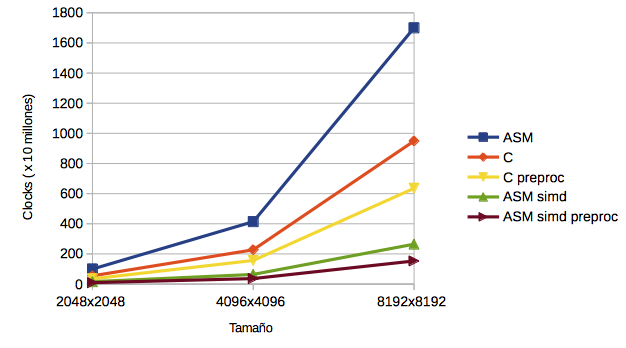
\includegraphics[width=\linewidth]{imgs/ldrTotales2.png}
	\end{minipage}\hfill
\end{figure}
 

\newpage

A su vez pudimos observar el poder de la optimizacion de C, ya que sin ningun esfuerzo de parte del programdor se obtiene una ganacia muy interesante, sobrepazando inclusive la version realizada en asm que no utilizaba instrucciones de SIMD.


\begin{figure}[!h]
	\centering
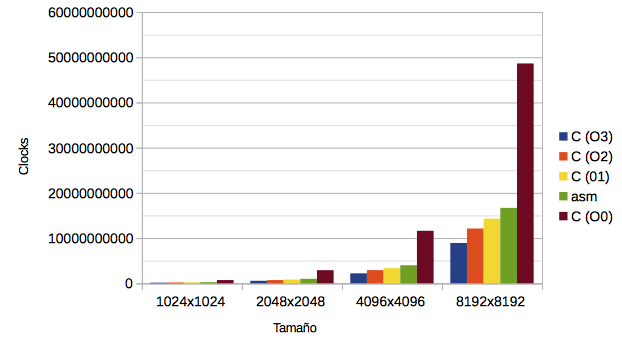
\includegraphics[width=300px]{imgs/ldrOptC.png}
\end{figure}




Dentro de los experimentos que decidimos realizar, nos preguntamos si existiria alguna diferencia en el el tiempo utilizado por los algoritmos dependiendo del parametro alpha, dado que se utiliza para multiplicar cada pixel.
Es interesante ver como se ve en el resultado de esta imagen, que para el valor de alpha=0, la cantidad de clocks utilizado, por los algoritmos que utilizan floats para la multiplicacion, diminuye significativamente. 
De esto se pueden sacar varias conclusiones interesantes, por un lado que la multiplicacion por el alpha consume una parte muy importante del tiempo total utilizado por el algoritmo.
Que si el valor es 0, el procesador resuelve inmediatamente el resultado y ademas que para el resto de los valores, no hay diferencia segun el valor por el cual se multiplique.

\begin{figure}[!h]
	\centering
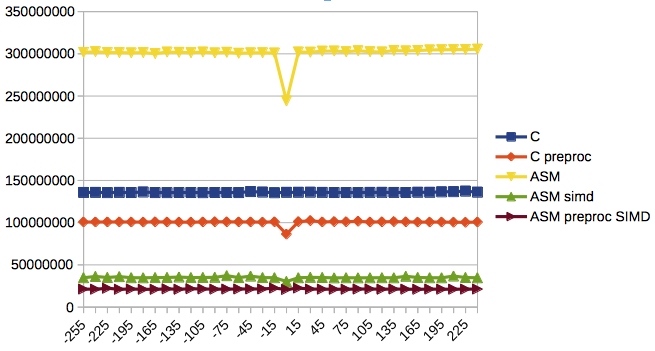
\includegraphics[width=300px]{imgs/comparacionLDR.png}
\end{figure}

